\documentclass[]{article}
\usepackage{lmodern}
\usepackage{amssymb,amsmath}
\usepackage{ifxetex,ifluatex}
\usepackage{fixltx2e} % provides \textsubscript
\ifnum 0\ifxetex 1\fi\ifluatex 1\fi=0 % if pdftex
  \usepackage[T1]{fontenc}
  \usepackage[utf8]{inputenc}
\else % if luatex or xelatex
  \ifxetex
    \usepackage{mathspec}
  \else
    \usepackage{fontspec}
  \fi
  \defaultfontfeatures{Ligatures=TeX,Scale=MatchLowercase}
\fi
% use upquote if available, for straight quotes in verbatim environments
\IfFileExists{upquote.sty}{\usepackage{upquote}}{}
% use microtype if available
\IfFileExists{microtype.sty}{%
\usepackage{microtype}
\UseMicrotypeSet[protrusion]{basicmath} % disable protrusion for tt fonts
}{}
\usepackage[unicode=true]{hyperref}
\hypersetup{
            pdfborder={0 0 0},
            breaklinks=true}
\urlstyle{same}  % don't use monospace font for urls
\usepackage{graphicx,grffile}
\makeatletter
\def\maxwidth{\ifdim\Gin@nat@width>\linewidth\linewidth\else\Gin@nat@width\fi}
\def\maxheight{\ifdim\Gin@nat@height>\textheight\textheight\else\Gin@nat@height\fi}
\makeatother
% Scale images if necessary, so that they will not overflow the page
% margins by default, and it is still possible to overwrite the defaults
% using explicit options in \includegraphics[width, height, ...]{}
\setkeys{Gin}{width=\maxwidth,height=\maxheight,keepaspectratio}
\IfFileExists{parskip.sty}{%
\usepackage{parskip}
}{% else
\setlength{\parindent}{0pt}
\setlength{\parskip}{6pt plus 2pt minus 1pt}
}
\setlength{\emergencystretch}{3em}  % prevent overfull lines
\providecommand{\tightlist}{%
  \setlength{\itemsep}{0pt}\setlength{\parskip}{0pt}}
\setcounter{secnumdepth}{0}
% Redefines (sub)paragraphs to behave more like sections
\ifx\paragraph\undefined\else
\let\oldparagraph\paragraph
\renewcommand{\paragraph}[1]{\oldparagraph{#1}\mbox{}}
\fi
\ifx\subparagraph\undefined\else
\let\oldsubparagraph\subparagraph
\renewcommand{\subparagraph}[1]{\oldsubparagraph{#1}\mbox{}}
\fi

% set default figure placement to htbp
\makeatletter
\def\fps@figure{htbp}
\makeatother


\date{}

\begin{document}

\emph{Frattura dello scafoide}

Le fratture dello scafoide sono fratture un po' particolari: lo scafoide
è un osso \emph{quasi completamente ricoperto da cartilagine(ad
eccezione dei punti di inserzione dei legamenti)} con una
\emph{vascolarizzazione retrograda di tipo terminale}. Per queste due
ragioni fratture di quest'osso guariscono con maggiore difficoltà.

La \textbf{prognosi} di guarigione dipende da diversi fattori:

\begin{enumerate}
\def\labelenumi{\arabic{enumi}.}
\item
  \textbf{Sede della lesione:} le fratture del polo prossimale
  guariscono con maggiore difficoltà, rispetto a quelle del terzo medio
  e del polo distale.
\end{enumerate}

\begin{enumerate}
\def\labelenumi{\arabic{enumi}.}
\item
  \textbf{Velocità della diagnosi:} molto spesso non sono diagnosticate
  immediatamente, ma a distanza di due/tre settimane, anche un mese, e
  non attraverso la radiografia normale, ma attraverso TAC (\emph{in
  questo caso la frattura può essere già andata incontro ad evoluzione
  in pseudoartrosi).}
\end{enumerate}

Molto spesso non vengono neanche studiate: il paziente ha dolore in
corrispondenza della tabacchiera anatomica, ma non va dal medico. A
distanza di sei mesi, un anno il dolore persiste, viene fatto un Rx e si
vede così una frattura non diagnosticata, che è andata incontro a
pseudoartrosi.

\begin{enumerate}
\def\labelenumi{\arabic{enumi}.}
\item
  \textbf{Caratteristiche del paziente:} più o meno giovane, più o meno
  attivo.
\end{enumerate}

Molto importanti sono anche le \emph{comorbilità}, che possono
influenzare di base una normale guarigione della frattura.

I pazienti fumatori, i pazienti con problematiche internistiche, come
diabete, ipertensione, ipertiroidismo vanno incontro a una guarigione
più lenta.

\begin{enumerate}
\def\labelenumi{\arabic{enumi}.}
\item
  \textbf{Adeguatezza del trattamento:} se si tratta incruentemente
  (ossia con un gesso) una frattura che dovrebbe essere operata, il
  risultato sarà peggiore.
\end{enumerate}

Allo stesso tempo anche un intervento chirurgico non adeguato può
influenzare negativamente la prognosi.

In più del 95\% dei casi questo tipo di fratture dei casi vengono
trattate incruentemente con l'applicazione di un apparecchio gessato.

È importante ricordare che in ortopedia molto spesso \emph{i segni
clinici di consolidazione}, ossia una riduzione della sintomatologia
dolorosa, \emph{precedono i segni radiografici}.

\emph{Epidemiologicamente, le fratture dello scafoide carpale sono
fratture che si riscontrano nel \emph{giovane adulto}, con una
prevalenza per il \emph{sesso maschile}, ed in una bassa percentuale dei
casi (\textbf{2-3\%}) può essere \emph{bilaterale}, interessando
prevalentemente il lato dominante del corpo, e nell'85\% dei casi sono
lesioni isolate, mentre nel restante 15\% dei casi sono associate ad
altre lesioni della mano e del polso (ad esempio fratture del radio o
lesioni dei legamenti intercarpali).}

\emph{Il meccanismo traumatico alla base è in genere collegato con
\emph{traumi in cui la mano viene appoggiata in modo particolare, ossia
quando c'è una caduta sul palmo della mano in iperestensione}: questo
movimento fa sì che il corpo dello scafoide si incunei in corrispondenza
della corrispondente superficie articolare del radio, così che si
sviluppa una sorta di meccanismo a leva che causa la frattura dello
scafoide.}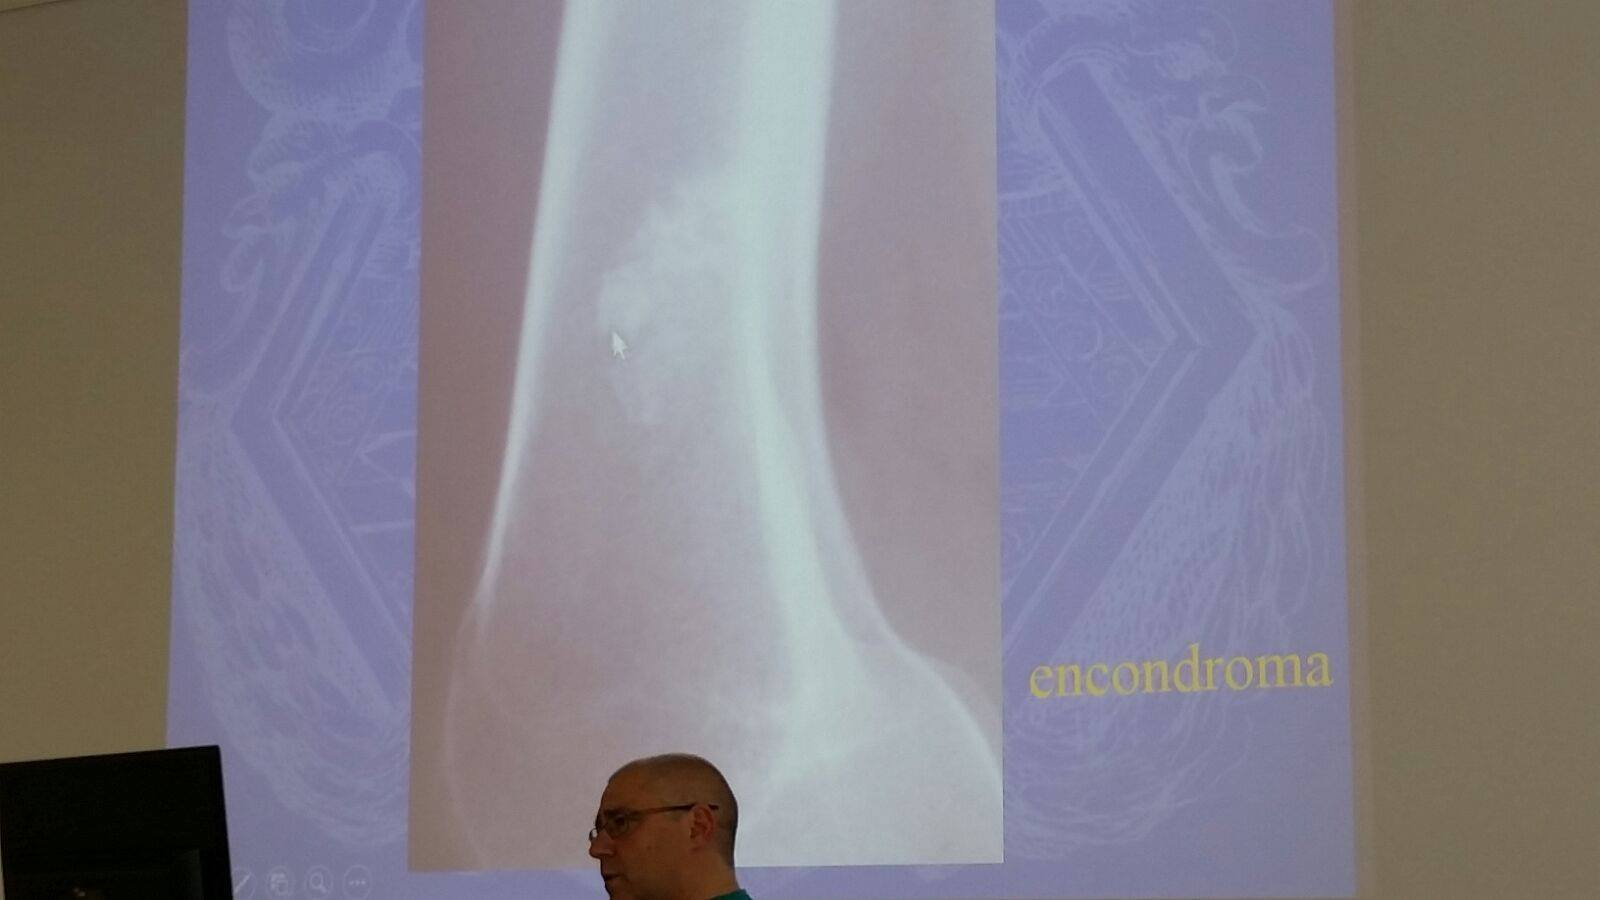
\includegraphics[width=3.54306in,height=2.65625in]{media/image1.jpeg}

\textbf{Le fratture dello scafoide posso essere divise in due tipi:}

\begin{itemize}
\item
  \emph{fratture a prognosi favorevole}: fratture \textbf{composte} e
  che interessano \textbf{polo distale e terzo medio} dello scafoide.
\end{itemize}

Nella maggior parte dei casi questo tipo di fratture guariscono con un
trattamento incruento:

\begin{itemize}
\item
  in passato si faceva un gesso lungo, \textbf{brachio-metacarpale con
  primo dito incluso} (gomito flesso a 90° fissato), che dopo un mese
  veniva sostituito con un gesso più corto.
\end{itemize}

\begin{itemize}
\item
  oggi si preferisce invece fin da subito un gesso più corto,
  \textbf{antibrachio-metacarpale}, cioè dalla fine dell'avambraccio
  fino ai metacarpi con primo dito incluso. Il gomito risulta libero.
\end{itemize}

\begin{quote}
Questo apparecchio gessato viene tenuto per più tempo rispetto a quelli
applicati per altri tipi di frattura, proprio perché lo scafoide tende a
guarire più lentamente. Quindi se di solito un gesso di polso viene
tenuto per 30-35-40 giorni, un gesso di scafoide rimane circa venti
giorni in più.

Una volta rimosso il gesso, si fa una \emph{lastra di controllo}: si
controlla che la frattura non si sia scomposta, si vede se ci sono
iniziali segni di consolidazione anche radiografica (formazione di
\textbf{callo osseo}) e in un secondo tempo si provvede a fare della
fisioterapia e della riabilitazione.
\end{quote}

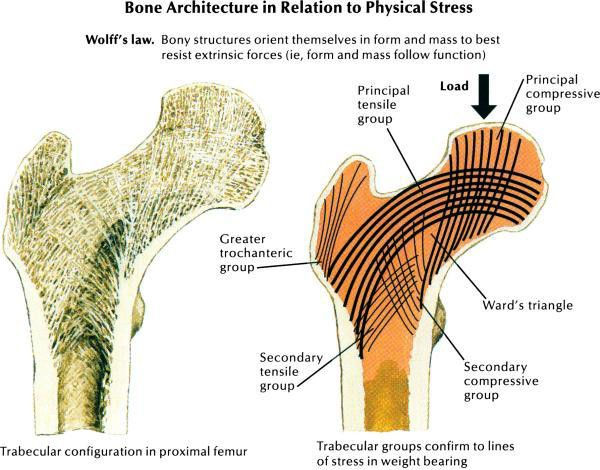
\includegraphics[width=2.76389in,height=2.07222in]{media/image2.jpeg}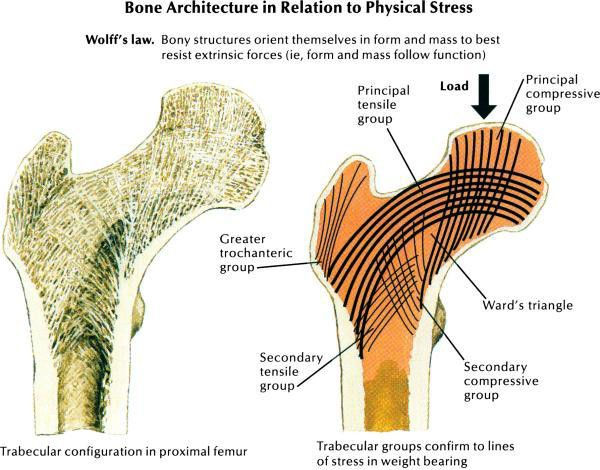
\includegraphics[width=2.78194in,height=2.08472in]{media/image3.jpeg}

\begin{itemize}
\item
  \emph{Fratture a prognosi sfavorevole}: fratture \textbf{scomposte} di
  qualsiasi segmento e quelle del \textbf{polo prossimale}.
\end{itemize}

Di solito sono trattate chirurgicamente: si esegue una \textbf{sintesi},
ossia una stabilizzazione della frattura previa riduzione, con una vite
in compressione. La vite può essere applicata \emph{a cielo aperto} (si
taglio, si espone la frattura, si riduce e poi si fa la sintesi con una
vita) o in modo \emph{percutaneo}, sfruttando un filo guida per inserire
la vite all'interno dello scafoide attraverso delle piccole incisioni.

Questo in linea di massima è il protocollo terapeutico delle fratture
dello scafoide.

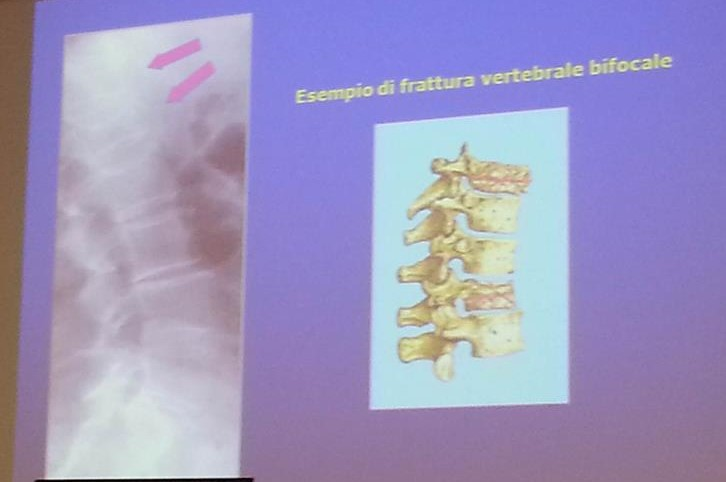
\includegraphics[width=2.78819in,height=2.09028in]{media/image4.jpeg}

\emph{Complicanze}

Lo scafoide, come già detto, è un osso molto particolare. In caso di
frattura va in contro ad una \textbf{crisi vascolare} e più facilmente
può andare in contro a complicanze:

\begin{enumerate}
\def\labelenumi{\arabic{enumi}.}
\item
  \emph{Ritardo di consolidazione e pseudoartrosi} dello scafoide, per
  una mancata vascolarizzazione e un rallentamento o un blocco dei
  normali processi biologici che permettono la guarigione della frattura
  stessa.
\end{enumerate}

\begin{enumerate}
\def\labelenumi{\arabic{enumi}.}
\item
  \emph{Necrosi ossea ischemica}, se l'afflusso di sangue si riduce
  drasticamente.
\item
  \emph{Artrosi secondaria post-traumatica}, soprattutto se non viene
  fatta una riduzione anatomica. Essendo quest'osso ricoperto da
  cartilagine e articolato con il radio distale e le ossa del carpo, una
  mancata corretta riduzione può predisporre all'insorgenza di
  un'artrosi post traumatica più facilmente che in caso di fratture in
  altre sedi.
\end{enumerate}

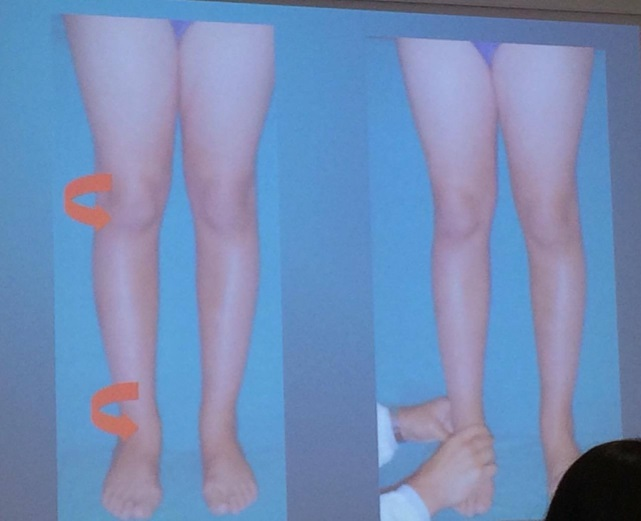
\includegraphics[width=3.49792in,height=2.62292in]{media/image5.jpeg}

Es (imm1): Rx di pseudoartrosi conseguente a mancata consolidazione di
una frattura del terzo medio dello scafoide: osso è bianco sul bordo e
si vede ancora la rima di frattura.

Es (imm2): RM con una necrosi del polo prossimale dello scafoide.

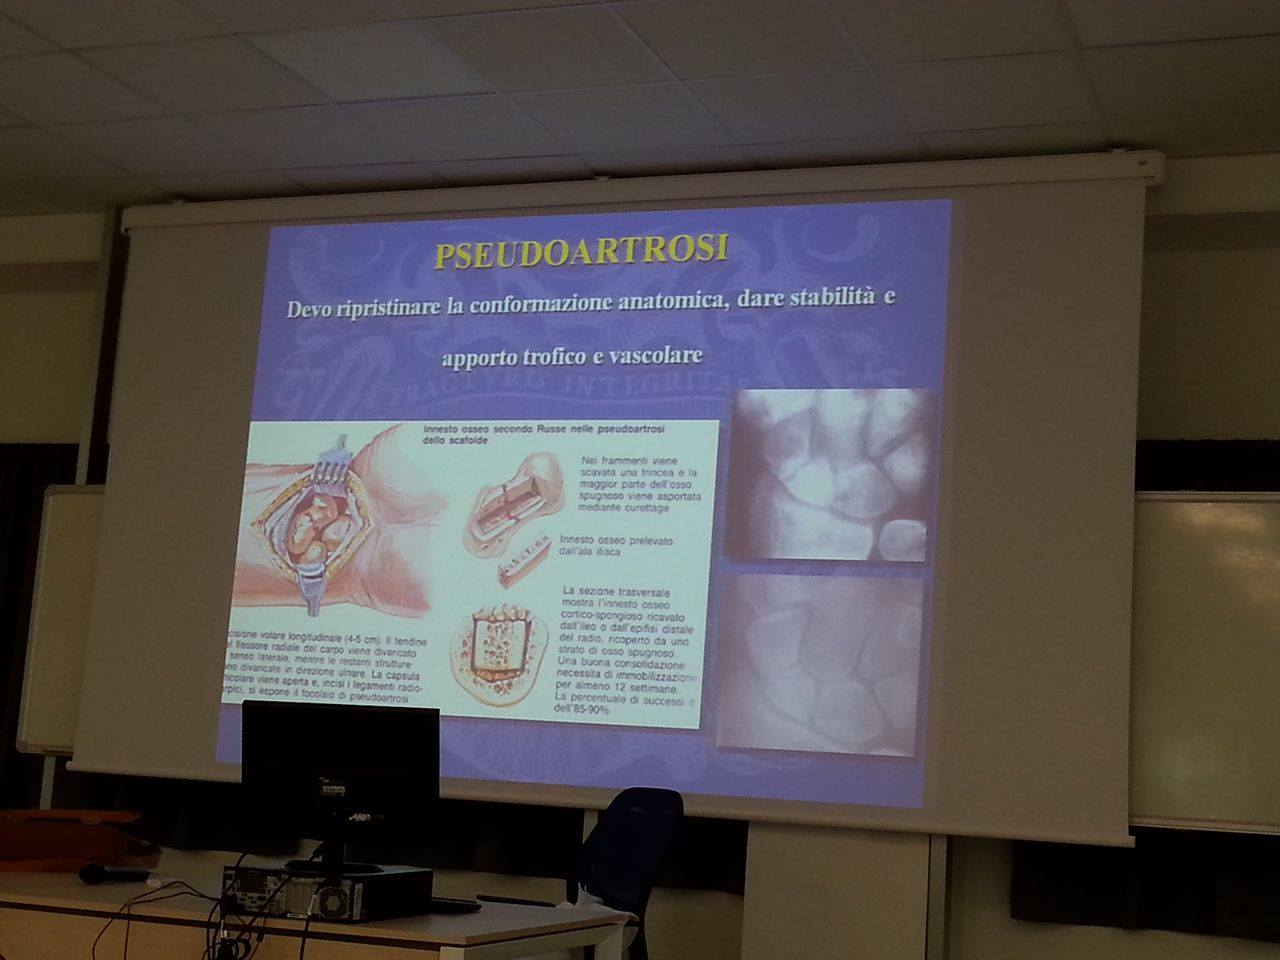
\includegraphics[width=3.45556in,height=2.59028in]{media/image6.jpeg}

Di fronte a una pseudoartrosi di scafoide il trattamento è uguale a
quello delle altre tipologie di pseudoartrosi.

La \textbf{psuedoartrosi} è una condizione di frattura che non è
consolidata e non consoliderà assolutamente.

Per trattarla è necessario:

\begin{itemize}
\item
  aprire il focolaio di pseudoartrosi,
\item
  ripulirlo dal tessuto cicatriziale, connettivo, fibroso che si è
  formato,
\item
  ripristinare la conformazione anatomica normale,
\item
  far sanguinare l'osso, in modo tale che si riinizi un normale processo
  biologico di guarigione.
\end{itemize}

Si può inserire all'interno del focolaio di pseudoartrosi dell'osso, di
solito prelevato da sé stessi, facendo un \emph{innesto osseo}. Si
preleva osso corticale e osso spongioso (ricco di cellule non
differenziate, staminali, che possono stimolare la cascata della
guarigione ossea) e il tutto viene messo all'interno del focolaio e poi
fissato attraverso dei fili metallici di Kirschner o delle viti.

Il miglior sito di prelievo è di solito la \emph{cresta iliaca}, dove è
possibile prelevare grosse quantità di osso corticale e spongioso.
Durante il prelievo bisogna stare attenti a non ledere i nervi, come il
nervo femoro-cutaneo laterale, che passa a cavaliere sopra la cresta
iliaca e che deve essere isolato e protetto per evitare dei neuromi
dolorosi lungo il decorso di questo nervo.

Altri siti donatori sono: il radio distale, l'olecrano e la tibia
prossimale, anche se dal punto di vista quali-quantitativo la sede di
prelievo migliore è la cresta iliaca.

Per favorire la guarigione è quindi necessario:

\begin{itemize}
\item
  pulizia del focolaio,
\end{itemize}

\begin{itemize}
\item
  la restitutio dell'anatomia normale,
\item
  stabilità conferita da viti o fili metallici
\item
  un buon apporto trofico e vascolare, dato da pulizia e apposizione di
  cellule ossee.
\end{itemize}

\emph{Fratture del polso}

Le fratture del polso sono fratture molto frequenti:

\begin{itemize}
\item
  prevalentemente nella popolazione anziana, spesso legate ad
  osteoporosi.
\end{itemize}

\begin{itemize}
\item
  sono frequenti anche nel bambino, con fratture a legno verde
\item
  nei traumi ad alta energia nei giovani adulti.
\end{itemize}

Interessano \emph{l'epifisi ditale di ulna e del radio} e posso essere
\emph{intra o extra-articolari} a seconda che la linea di frattura
interessi o meno la cartilagine articolare di radio e ulna.

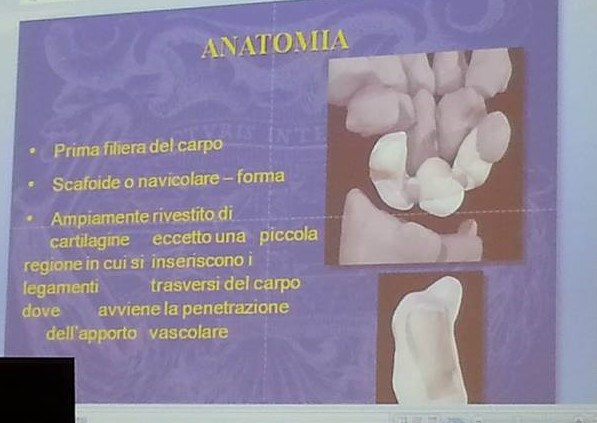
\includegraphics[width=3.25000in,height=2.43472in]{media/image7.jpeg}

Esistono \textbf{due tipi} di frattura:

\begin{itemize}
\item
  \textbf{Frattura di tipo COLLES:} la più frequente (85-90\%),
  soprattutto negli anziani, per un trauma da \emph{caduta sul palmo
  della mano}, con la mano atteggiata \emph{in iperestensione dorsale}
  (simile a modalità di frattura dello scafoide).
\end{itemize}

Vi è una scomposizione del radio distale e migrazione dorsale dei
frammenti ossei. Può interessare anche il processo stiloideo dell'ulna.

Il reperto all'esame obiettivo è il cosiddetto \textbf{polso a dorso di
forchetta}.

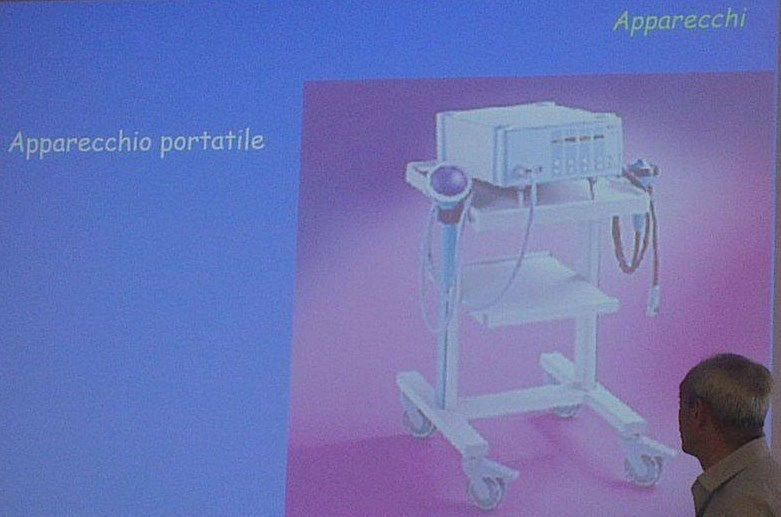
\includegraphics[width=3.12500in,height=2.34167in]{media/image8.jpeg}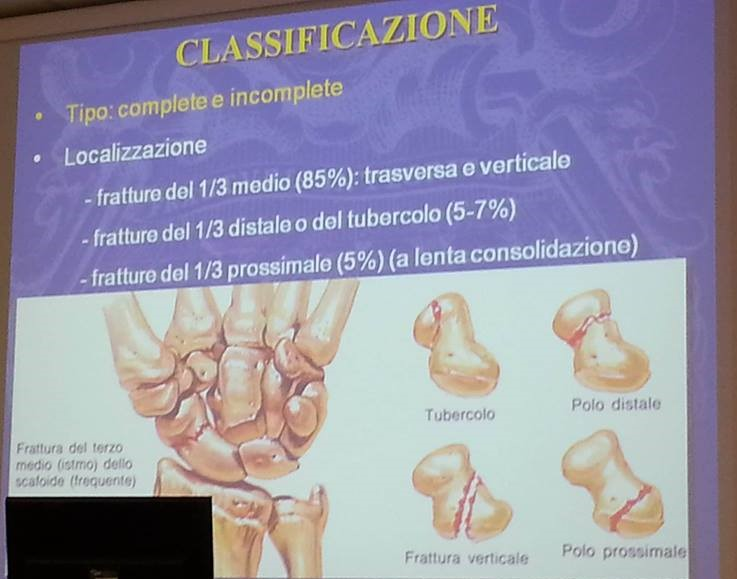
\includegraphics[width=3.12569in,height=2.34167in]{media/image9.jpeg}

\begin{itemize}
\item
  \textbf{Fratture di tipo Goyrand:} sono fratture meno frequenti.
  Avvengo per \emph{caduta sul dorso della mano}, con un meccanismo
  eziopatogenetico opposto rispetto alle fratture di Colles.
\end{itemize}

La frattura si estrinseca nello stesso punto e il \emph{radio distale si
scompone volarmente}, verso il palmo della mano.

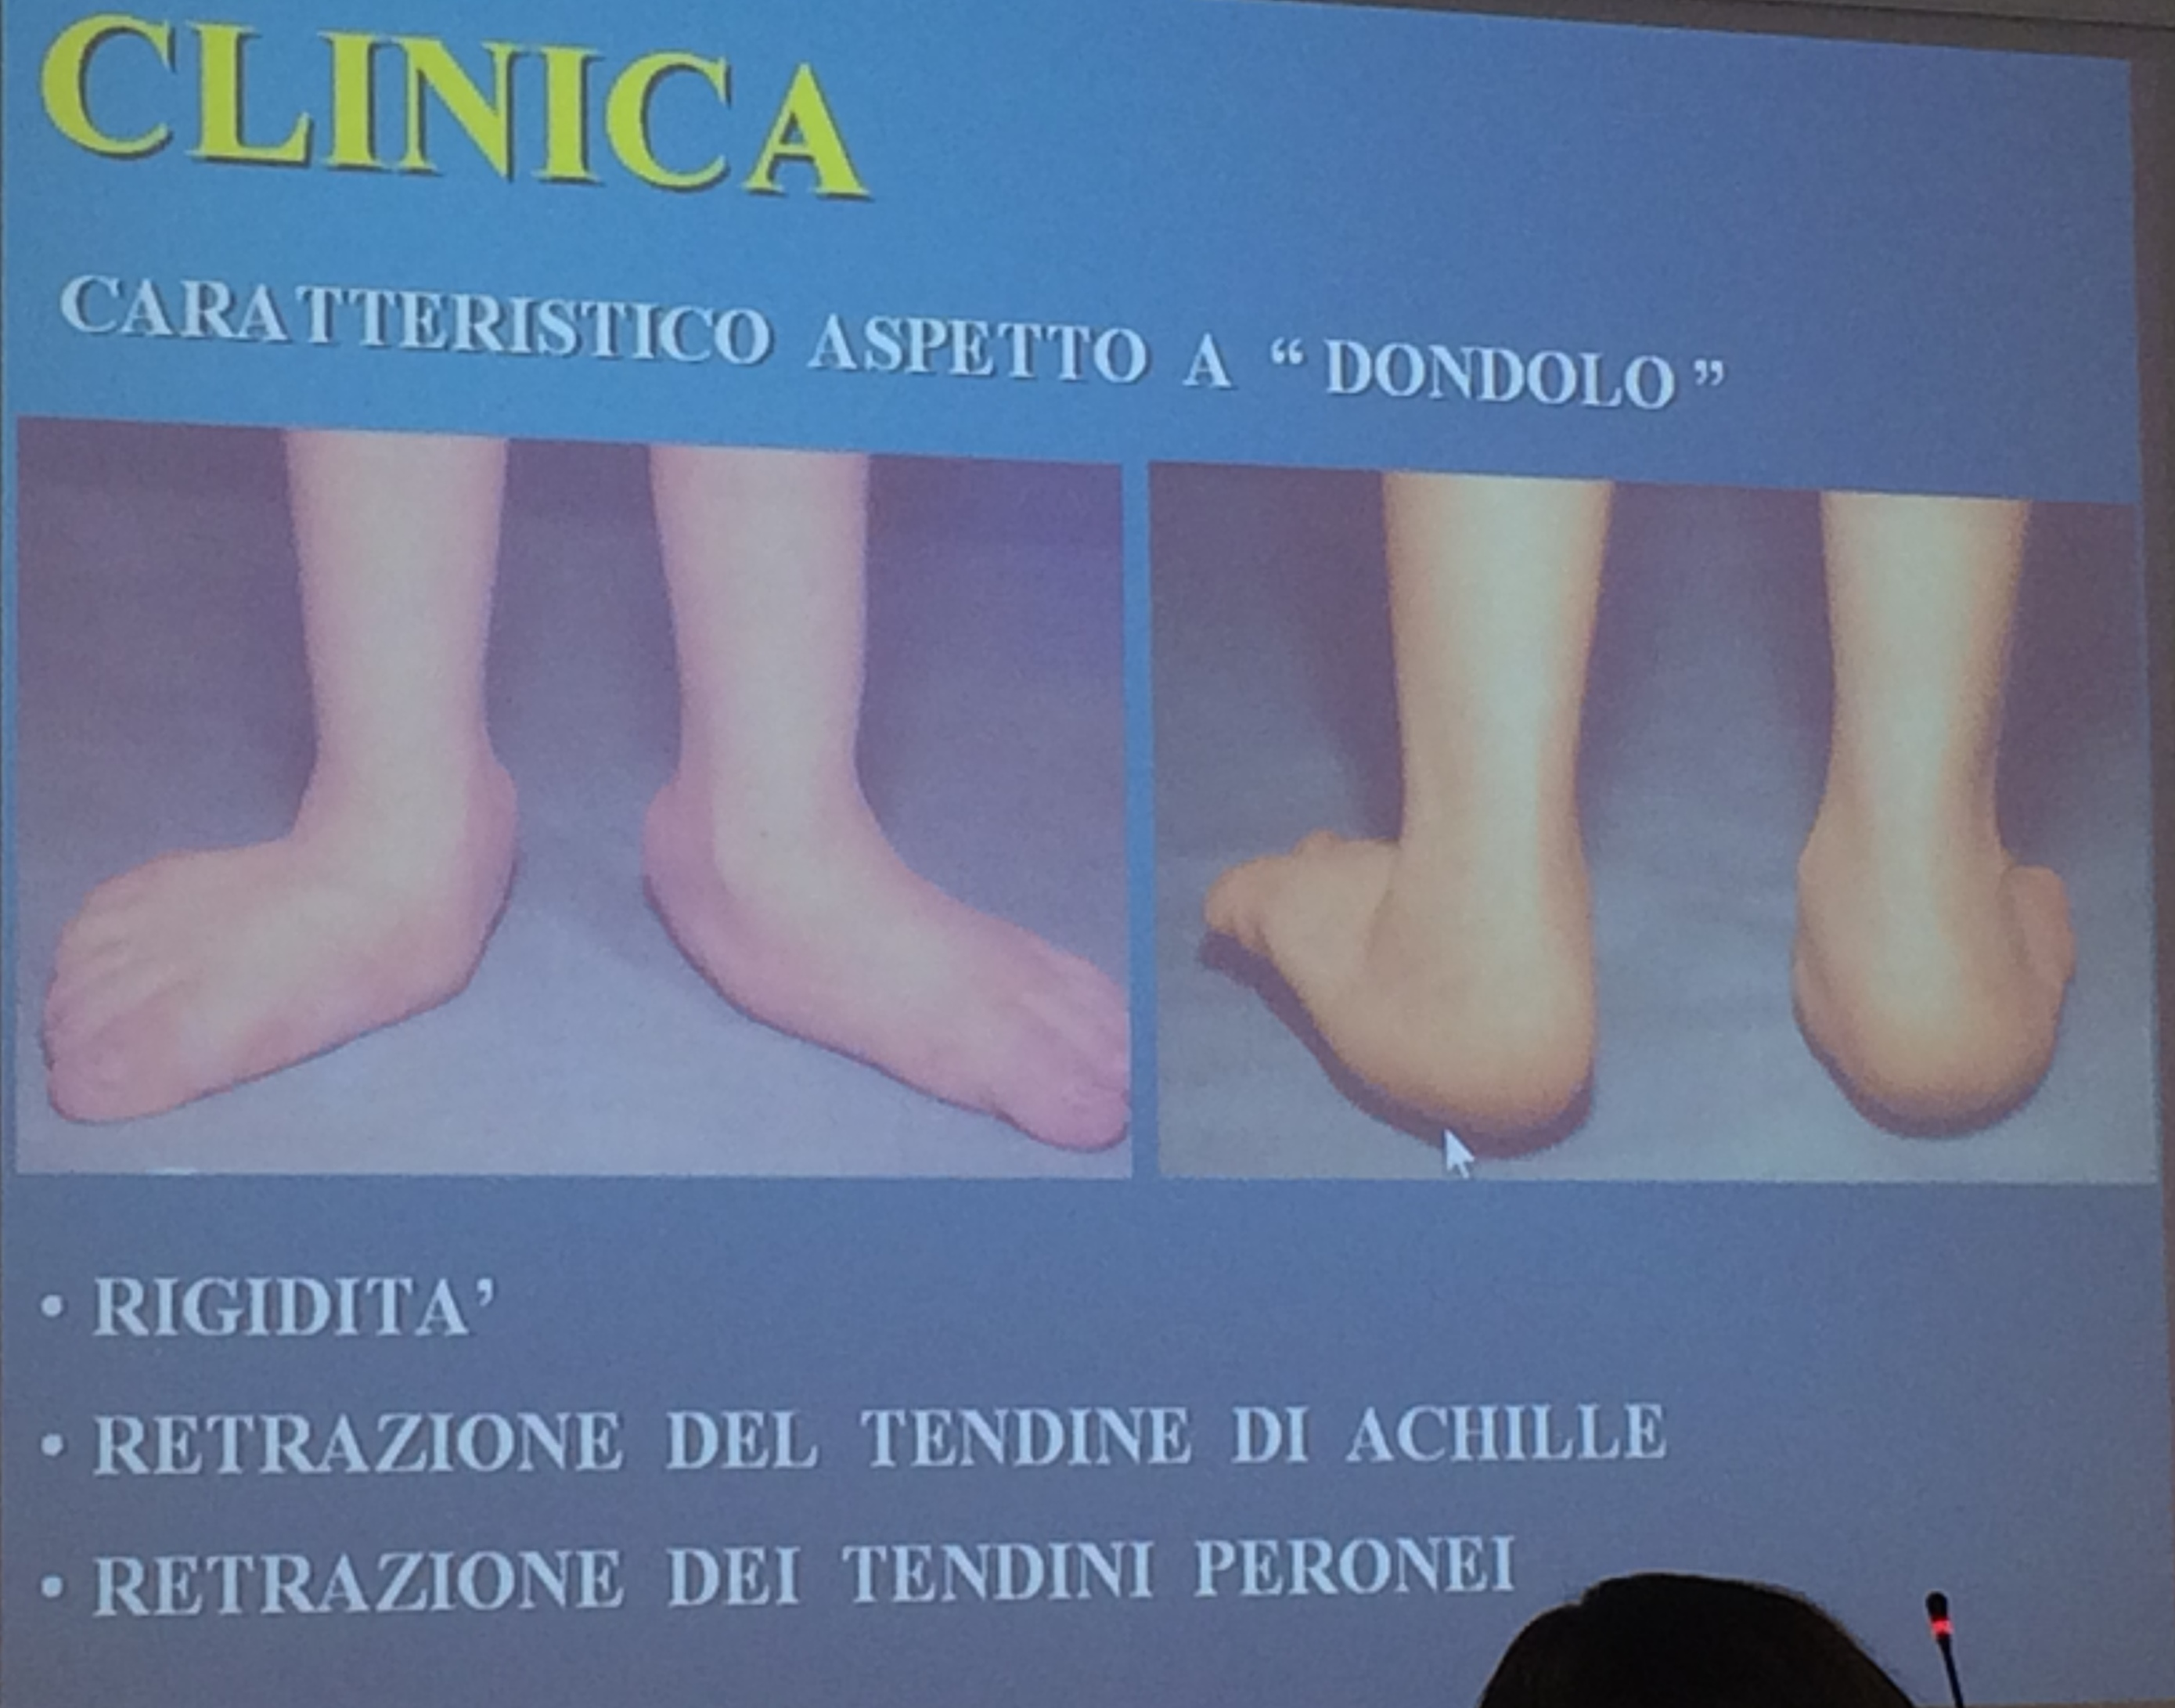
\includegraphics[width=3.27014in,height=2.45069in]{media/image10.jpeg}

\emph{Trattamento}

Nel caso di fratture del polso, in PS bisogna sempre fare un
\emph{tentativo di riduzione} in anestesia locale, a cui segue
l'applicazione di un \emph{apparecchio gessato}.

Il gesso viene subito controllato con \textbf{radiografia}, per
verificare che la riduzione sia efficace o meno. Devono essere
controllate radiologicamente in gesso dopo 7, 14 e a volte anche 21
giorni dall'evento. Questo perché questi tipi di fratture soprattutto
(ma in realtà ogni tipo di frattura trattata con il gesso), possono, in
questa sequenza temporale, andarsi a \textbf{scomporre}, perdendo la
riduzione.

Questo avviene perché il segmento immobilizzato, sgonfiandosi, può non
essere ben contenuto nel gesso e i micromovimenti che si vengono a
creare determinano la perdita della riduzione.

In linea di massima nel momento in cui si perde una riduzione, si dà
un'\emph{indicazione chirurgica}. La \textbf{perdita della riduzione} è
indice di una \textbf{frattura instabile} ed è quindi, soprattutto nel
giovane, indicato un intervento chirurgico.

A volte negli individui anziani, che mal sopporterebbero un intervento
chirurgico, si può provare a rifare la riduzione.

Le fratture di \emph{tipo Goyrand} sono di solito \emph{più difficili da
ridurre} e molto più frequentemente vanno incontro ad un intervento
chirurgico.

Questo di solito prevede una \textbf{riduzione} e \textbf{osteosintesi a
cielo aperto} con placche e viti, a volte anche associato a fili
metallici percutanei.

In casi ancora più selezionati, come nelle \emph{fratture esposte} e
nelle \emph{fratture pluriframmentarie} del radio distale, dove non si
riesce a ridare stabilità con placche e viti, può essere indicato
utilizzare uno \textbf{stabilizzatore esterno con distrazione}.

Viene applicato con due fiches a livello del metacarpo e due fiches in
corrispondenza della metafisi distale del radio: la distrazione fa sì
che i legamenti radio-carpici, venendo stirati, tendano a ridurre a poco
a poco la frattura.

Viene sfruttato il principio della \emph{legamentotassi}, ossia la
trazione legamentosa determina una riduzione non anatomica, ma comunque
soddisfacente, della frattura.

Al fissatore esterno può anche essere associato l'uso di fili metallici,
\emph{fili di Kirschner} \emph{percutanei}.

Il fissatore esterno viene mantenuto per almeno due mesi. Dopo un mese
può essere \textbf{dinamizzato}, cioè rimane in distrazione, ma può
essere permesso il movimento.

\emph{Altre lesioni traumatiche della mano}

\emph{MALLET FINGER}

Il MALLET FINGER (o dito a martello) si verifica quando si riceve un
urto direttamente sull'estremità distale del dito e \emph{l'ultima
falange assume un deformità a martello} (di solito giocando a basket,
pallavolo,
calcio).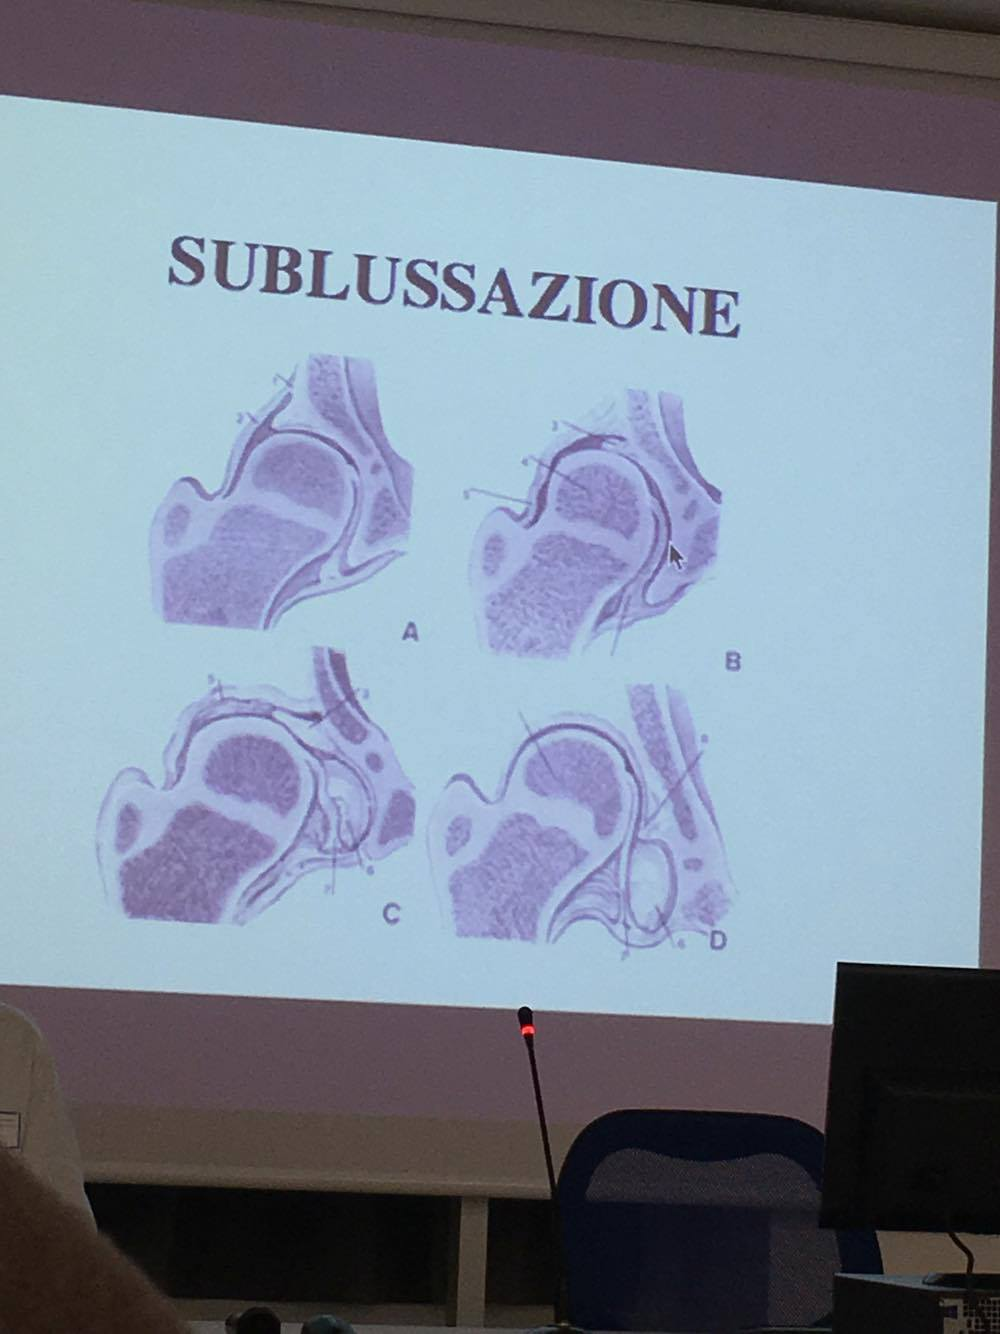
\includegraphics[width=2.52083in,height=1.89028in]{media/image11.jpeg}

Un deformità a martello può essere dovuta a due cause:

\begin{itemize}
\item
  una \emph{rottura sottocutanea dell'estensore del dito}, che di solito
  di inserisce a livello della falange distale
\item
  \emph{un'avulsione del tendine} che stacca l'osso sempre a livello
  della falange distale.
\end{itemize}

Quando arriva al PS un paziente con un dito a martello bisogna subito
fare un RX per vedere che sotto non ci sia una frattura della falange
distale.

\begin{itemize}
\item
  Il dito a martello associato a una frattura si chiama \textbf{lesione
  di Segond}.
\end{itemize}

\begin{itemize}
\item
  Il dito a martello non associato a frattura si chiama semplicemente
  \textbf{rottura sottocutanea dell'estensore del dito a livello della
  falange distale}.
\end{itemize}

\emph{Trattamento}

\begin{enumerate}
\def\labelenumi{\arabic{enumi}.}
\item
  Qualora vi sia solo una lesione a livello dell'estensore il
  trattamento è solitamente incruento e consiste nell'applicazione di
  una \textbf{stecca di Zimmer} o in plastica o metallica, che
  \emph{mantiene il dito iperesteso} all'interfalangea distale.
\end{enumerate}

Ciò permette al tendine immobilizzato di cicatrizzare.

\begin{quote}
L'immobilizzazione deve essere mantenuta almeno 50-55 giorni.

Ogni tanto il paziente può togliere la stecca, con l'accortezza di
mantenerlo iperesteso (o appoggiandolo sul tavolo o con l'altra mano).
\end{quote}

Nel momento in cui la stecca viene tolta progressivamente il paziente
può iniziare la \textbf{fisioterapia} per riacquisire l'articolarità.

Bisogna informare il paziente, che verosimilmente un po' di flessione
dell'ultima falange rimarrà alla rimozione della stecca, ma anche se dal
punto di vista estetico non sarà bellissima, dal punto di vista
funzionale vi sarà un completo recupero.

\begin{enumerate}
\def\labelenumi{\arabic{enumi}.}
\item
  Qualora invece siano associate delle fratture (lesione di Segond)
  bisogna valutare quanto \emph{osso} risulta essere \emph{avulso},
  osservando una proiezione radiografica laterale.
\end{enumerate}

Se il pezzo d'osso è superiore al 25\% dell'altezza del dito stesso, il
trattamento è di solito chirurgico e consiste nella \textbf{reinserzione
del frammento} nella propria sede.

Può essere fatto con microviti o fili metallici.

Si cerca comunque di evitare l'intervento chirurgico, perché si tratta
di una zona cutanea molto delicata e la ferita può fare fatica a guarire

\emph{LESIONE DI STENER}

La LESIONE DI STENER è la \emph{rottura del legamento collaterale ulnare
in corrispondenza della prima articolazione metacarpo-falangea} della
mano.

Quest'articolazione è stabilizzata, oltre che dalla capsula articolare,
da due legamenti: il legamento \textbf{collaterale ulnare} e il
legamento \textbf{collaterale radiale}.
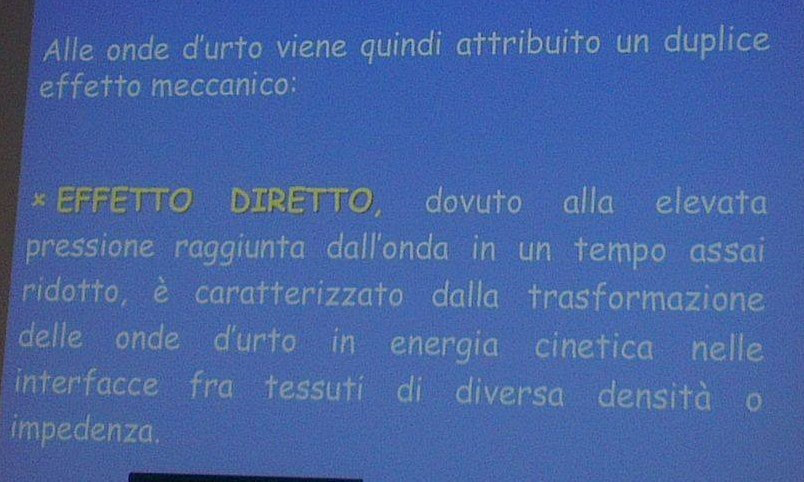
\includegraphics[width=2.08681in,height=1.52153in]{media/image12.jpeg}

Quello ulnare è molto importante perché garantisce la presa di forza
della mano.

Si rompe soprattutto in ambito sportivo: per esempio sciando, nel tennis
quando il dito rimane incastrato nella racchetta o negli incidenti in
moto, quando il dito rimane vincolato al freno o all'acceleratore.

I pazienti presentano \textbf{dolore} e \textbf{tumefazione} localizzata
e la manovra in stress radiale determina dolore e sensazione manuale di
instabilità. Il dolore può essere molto forte e queste manovre posso
quindi essere fatte iniettando un po' di anestetico locale.

Questa sensazione manuale di \textbf{instabilità} può essere confermata
attraverso delle radiografie in stress bilaterali, fatte da un bravo
tecnico radiologo.

Le radiografie mettono in evidenza l'apertura di questa articolazione
rispetto alla controlaterale.

\emph{Trattamento}

In un paziente giovane, attivo, con difficoltà della forza di presa in
acuto deve essere trattato \textbf{chirurgicamente} (non immediatamente,
ma nel giro di 3-4-5 giorni).

Si taglia, si scosta il ramo sensitivo del nervo radiale, per evitare di
lesionarlo e si riattacca il legamento con un'ancoretta a livello della
falange (sede più tipica di rottura).

Le lesioni sono nella maggior parte dei casi a livello della falange,
più raramente a livello della testa del metacarpo e ancora più raramente
lungo il suo decorso.

All'intervento segue \textbf{l'immobilizzazione} attraverso un
\emph{apparecchio gessato} per il primo dito o un \emph{tutore} su
misura per una ventina di giorni e poi una \textbf{rieducazione} di
almeno un mese e mezzo per recuperare la forza dei muscoli dell'eminenza
tenar e la forza di presa.

\end{document}
